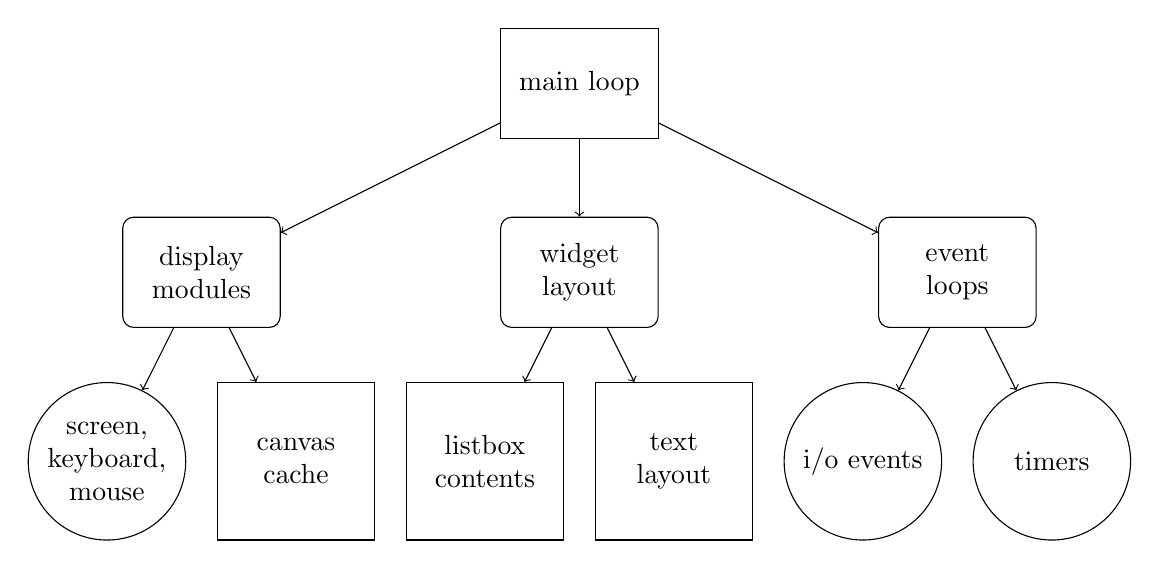
\begin{tikzpicture}[
  rectblock/.style = {rectangle, draw, inner sep = 0pt, align = flush center, minimum width = 2cm, minimum height = 1.4cm},
  roundblock/.style = {rectblock, rounded corners},
  circleblock/.style = {circle, draw, inner sep = 0pt, align = flush center, minimum size = 2cm},
  squareblock/.style = {rectblock, draw, align = flush center, inner sep = 0pt, minimum width = 2cm, minimum height = 2cm},
  x = 1.2cm,
  y = 0.8cm
]
  \node[rectblock]   (ml) at (7, 8) {main loop};
  \node[roundblock]  (dm) at (3, 5) {display\\modules};
  \node[roundblock]  (wl) at (7, 5) {widget\\layout};
  \node[roundblock]  (el) at (11, 5) {event\\loops};
  \node[circleblock] (skm) at (2, 2) {screen,\\keyboard,\\mouse}; 
  \node[squareblock] (cc) at (4, 2) {canvas\\cache};
  \node[squareblock] (lc) at (6, 2) {listbox\\contents};
  \node[squareblock] (tl) at (8, 2) {text\\layout};
  \node[circleblock] (io) at (10, 2) {i/o events};
  \node[circleblock] (ti) at (12, 2) {timers};
  
  \draw[->] (ml) -- (dm);
  \draw[->] (ml) -- (wl);
  \draw[->] (ml) -- (el);
  \draw[->] (dm) -- (cc);
  \draw[->] (dm) -- (skm);
  \draw[->] (wl) -- (lc);
  \draw[->] (wl) -- (tl);
  \draw[->] (el) -- (io);
  \draw[->] (el) -- (ti);
\end{tikzpicture}